\documentclass[fleqn]{article}
\usepackage[utf8x]{inputenc}
\usepackage{graphicx}
\usepackage{amsmath}
\usepackage[left=2cm,right=2cm,top=2cm,bottom=2cm,bindingoffset=0cm]{geometry}
\usepackage[russian]{babel}
\usepackage{fancyvrb}

\title{Лабораторная работа}
\begin{document}
\maketitle

\section*{Преобразование Хафа для детектирования линий}
\subsection*{Теоретическая справка}
В основе теории преобразования Хафа лежит утверждение, что любая точка двоичного изображения может быть частью некоторого набора возможных линий.

\begin{figure}[h]
\center{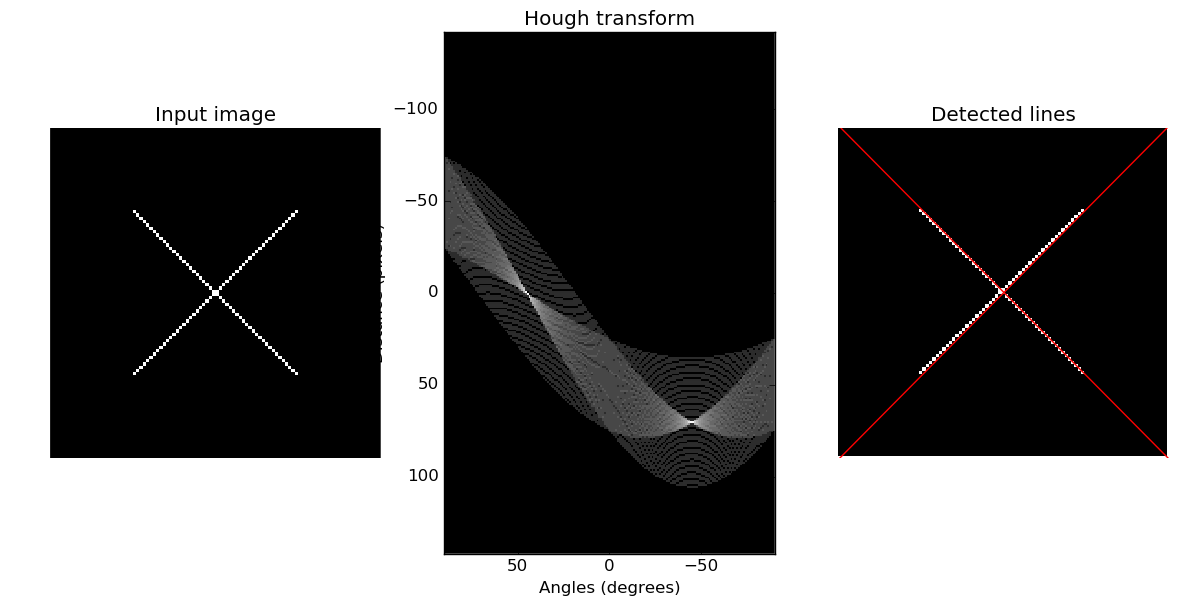
\includegraphics[width=0.5\linewidth]{ex1.png}}
\caption{Исходное изображение, соответсвующее ему фазовое пространство и
найденные линии}
\label{ris:image}
\end{figure}

Линия задается уравнением в полярных координатах: $x \cos(f) + y \sin(f) = R$, где $R$ --- длина перпендикуляра, опущенного на линию из начала координат, а $f$ --- угол между перпендикуляром и осью абсцисс, находится в пределах $[0,2 \pi]$. Через каждую точку $(x, y)$ изображения можно провести несколько прямых с разными $R$ и $f$, то есть каждой точке $(x, y)$ изображения соответствует набор точек в фазовом пространстве $(R, f)$, образующий синусоиду. Также каждой точке $(R_0, f_0)$ пространства $(R, f)$ можно поставить в соответствие счетчик, соответствующий количеству точек $(x, y)$, лежащих на прямой $x cos(f_0) + y sin(f_0) = R_0$. Непрерывное фазовое пространство переводится в дискретное вводом сетки на пространстве $(R, f)$, одной ячейке которой соответствует набор прямых с близкими значениями $R$ и $f$.

\subsection*{Задание}
Вам необходимо реализовать алгоритм поиска линий на изображении.
\begin{enumerate}
    \item Выделите края изображения с помощью фильтра Canny или фильтра Sobel.
    \item Создайте отдельную функцию houghlines, принимающую на вход изображение, шаг сетки, точность попадания точки на прямую и возвращающую матрицу фазового пространства Хафа. В рамках функции создайте матрицу для хранения фазового простанства Хафа. Для каждого контурного пикселя исходного изображения необходимо рассмотреть все возможные прямые, которые могут проходить через эту точку (угол наклона $f$ и расстояние от начала координат $R$). Если $ \Bigl|(y \sin(f) + x \cos(f)) - r \Bigr| < accuracy$, увеличиваем счетчик для этой точки фазового пространства.
    \item Визуализируйте полученное фазовое пространство.
    \item Преобразуйте точки фазового пространства с максимальным откликом в линии.
    \item Визуализируйте линии на исходном изображении.
    \item Подберите оптимальные параметры для тестовых изображений <<line1.png>>, <<line2.png>>, <<line3.png>>.
    \item Сравните работу написанного алгоритма с функцией cvHoughLines2 из
        библиотеки OpenCV или hough\_line из библиотеки scikits\_image.
\end{enumerate}

\section*{Преобразование Хафа для детектирования окружностей}
\subsection*{Задание}
Вам необходимо реализовать алгоритм окружностей на изображении.
\begin{enumerate}
    \item Выделите края изображения с помощью фильтра Canny или фильтра Sobel.
    \item Выпишите параметрическое уравнение окружности. Сколько параметров в него входит?
    \item Создайте отдельную функцию houghcircles, по аналогии с houghlines.
    \item Визуализируйте полученное фазовое пространство.
    \item Преобразуйте точки фазового пространства с максимальным откликом в окружности.
    \item Визуализируйте окружности на исходном изображении.
    \item Подберите оптимальные параметры для тестовых изображений <<circle1.png>>, <<circle2.png>>, <<circle3.png>>.
    \item Сравните работу написанного алгоритма с функцией hough\_circle из
        библиотеки scikits\_image.
\end{enumerate}

\end{document}
